%%%%%%%%%%%%%%%%%%%%%%%%%%
%                          %
% ----- INTRODUCTION ----- %
%                          %
%%%%%%%%%%%%%%%%%%%%%%%%%%

\section{Processus de test}

	Une fois toutes les parties du projet réalisées, à savoir l'extension navigateur, le serveur et l'interface, nous avons cherché des utilisateurs volontaires pour installer l'extension et l'utiliser pendant une période de 4 semaines. Bien qu'initialement prévue pour un grand panel d'utilisateurs, les restrictions temporelles ont limité la quantité d'utilisateurs que nous avons pu atteindre.

	Un total de 10 utilisateurs volontaires ont installé l'extension. Parmi eux, 8 ont été identifiés comme ayant une activité de navigation  sur Chrome assez grande pour contribuer à l'étude. (Ceux étant jugés inactifs totalisent moins de 10 minutes d'activité).

	\subsection{Inputs}

		En plus de récolter les données des utilisateurs et de les afficher, il leur a également été demandé de remplir quelques informations sur eux-même afin de pouvoir valider certains points de notre étude. Deux formulaires ont été mis en place à cette fin.

		\subsubsection{Centres d'intérêts}

			La figure~\ref{settings_image} montre un premier formulaire à remplir par l'utilisateur. Accessible via le lien vers la page "Settings", on lui demande ici de trouver et renseigner quelques uns de ces centres d'intérêt parmi une centaine.

			\begin{figure}[!h]
				\centering
				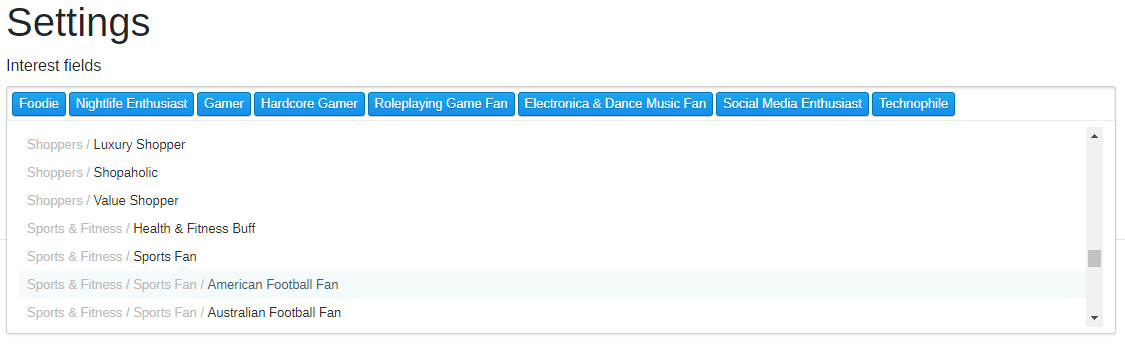
\includegraphics[height=0.32\textwidth]{images/design/pages/settings}
				\caption{Champ d'entrée des centres d'intérêts}
				\label{settings_image}
			\end{figure}

			Un maximum de 10 centres d'intérêts peuvent être définis. Le but de laisser à l'utilisateur entrer des centres d'intérêts est de pouvoir nous rendre compte si les topics que nous lui proposons sont proches de ces centres d'intérêt.

		\subsubsection{Association topic et intérêt}

			Une fois que l'utilisateur a défini des centres d'intérêt, il peut donner des informations sur les topics que nous lui suggérons sur la page Topics List (voir section \ref{topicslist}). La figure~\ref{choice} montre la fenêtre déroulante de sélection d'un centre d'intérêt pour un topic donné.

			\begin{figure}[!h]
				\centering
				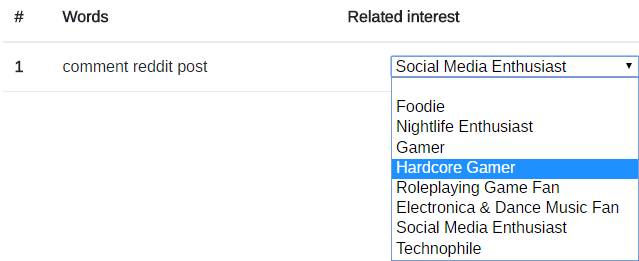
\includegraphics[height=0.32\textwidth]{images/results/choice}
				\caption{Sélection d'intérêt sur un topic}
				\label{choice}
			\end{figure}

			Il est demandé aux utilisateurs d'ajouter une association entre un topic et un intérêt lorsque cela semble lui faire sens. Ainsi, nous pouvons savoir quels topics de l'utilisateur nous avons réussi à identifier. En effet, lorsqu'un utilisateur associe un centre d'intérêt à un topic, celà signifie non seulement que le topic trouvé a du sens en soi, mais en plus qu'il est intéressant pour l'utilisateur.

			Sur l'échantillon de 8 personnes actives, 6 personnes ont ajouté des associations aux 20 topics proposés sur leur page. 

\section{Evaluation}

	Après une récolte des données sur environ 4 semaines, nous pouvons nous intéresser aux résultats que nous avons récoltés.

	\subsection{Modèles}

		Une première étape est de se pencher sur les modèles que nous avons généré sur la base des données elle-mêmes. Nous utilisons principalement deux algorithmes qui se basent sur le contenu des pages pour en déterminer leur thème : TF-IDF, et LDA.

		Ces modèles se basent sur le contenu des pages visitées des utilisateurs. Etant donné que nous ne récupérons pas directement le contenu de la page visitée par un utilisateur mais uniquement une partie de son URL, nous ne pouvons pas garantir que le contenu que nous récupérons d'une page soit effectivement le contenu que l'utilisateur voit sur son écran. En effet, beaucoup de pages web aujourd'hui sont liées à une application qui demande une authentification de l'utilisateur pour être affichée.

		Par exemple, une grande partie des pages d'un réseau social peuvent nécessiter la connexion de l'utilisateur pour être affichée.

		\subsubsection{TF-IDF}

			\paragraph{Résultats}

				Le fonctionnement de TF-IDF est décrit à la section \ref{analyse-tfidf}. Juger les résultats du calcul de TF-IDF sur des documents est une tâche non triviale. Cela revient principalement à vérifier manuellement que les mots ayant le poids le plus élevé pour certaines pages soit significatif de leur sujet.

				Intéressons-nous donc aux mots ayant le plus de poids trouvés pour les 20 pages les plus regardées, par exemple. Le tableau\ref{table-tfidf} illustre les 20 pages les plus regardées avec leurs mots associés, ainsi que plusieurs étapes amenant à une estimation finale de l'adéquation des mots trouvés avec le contenu de la page. Voici comment se lit le tableau :
				\begin{description}
					\item[URL] URL de la page concernée. Certaines URLs trop longues ont été raccourcies ici
					\item[Mot 1, 2, 3] 3 meilleurs mots dans l'orrdre décroissant décrivant la page selon TF-IDF.
					\item[Pub(lique)] Est-ce que la page nécessite une connexion afin d'accéder à son contenu principal.
					\item[Con(tenu)] Est-ce que le principal contenu de la page est textuel ?
					\item[Mot] Est-ce que chacun des mots trouvés sur la page fait sens dans une langue connue ?
					\item[Adé(quat)] Est-ce que l'ensemble des mots trouvés forme un potentiel résumé adéquat du contenu de la page ?
				\end{description}

				Les 4 premières colonnes (URL et 3 mots) proviennent de la base de données, tandis que les 4 dernières colonnes sont le résultat d'une évaluation manuelle des critères décrits. Un "OUI" dans une colonne indique que la page a passé le critère défini, contrairement à un "NON". Un "NON" dans une colonne entraîne automatiquement un "NON" dans les colonnes situées les plus à droite.

\begin{sidewaysfigure}
\centering
\caption{20 URLs les plus regardées et leurs meilleurs mots selon TF-IDF}
\label{table-tfidf}
\begin{tabular}{llllllll}
\textbf{URL}                                          & \textbf{Mot 1}  & \textbf{Mot 2}           & \textbf{Mot 3} & \textbf{Pub}           & \textbf{Con}            & \textbf{Mot}               & \textbf{Adé}            \\ \hline
\scriptsize \url{http://wdf.sdipi.ch/}                              & footprints      & digital                  & web            & \cellcolor[HTML]{9AFF99}OUI & \cellcolor[HTML]{9AFF99}OUI & \cellcolor[HTML]{9AFF99}OUI & \cellcolor[HTML]{9AFF99}OUI \\
\scriptsize \url{https://www.draw.io/}                                  & gmdl            & eng                      & proc           & \cellcolor[HTML]{9AFF99}OUI & \cellcolor[HTML]{FFCCC9}NON & \cellcolor[HTML]{FFCCC9}NON & \cellcolor[HTML]{FFCCC9}NON \\
\scriptsize \url{https://www.reddit.com/r/videos/}                      & submit          & load                     & report         & \cellcolor[HTML]{9AFF99}OUI & \cellcolor[HTML]{9AFF99}OUI & \cellcolor[HTML]{9AFF99}OUI & \cellcolor[HTML]{FFCCC9}NON \\
\scriptsize \url{https://www.google.co.uk/search}                       & eingabetaste    & suche                    & drücke         & \cellcolor[HTML]{9AFF99}OUI & \cellcolor[HTML]{FFCCC9}NON & \cellcolor[HTML]{FFCCC9}NON & \cellcolor[HTML]{FFCCC9}NON \\
\scriptsize \url{https://www.google.ch/search}                          & eingabetaste    & suche                    & drücke         & \cellcolor[HTML]{9AFF99}OUI & \cellcolor[HTML]{FFCCC9}NON & \cellcolor[HTML]{FFCCC9}NON & \cellcolor[HTML]{FFCCC9}NON \\
\scriptsize \url{http://game110.idlekiller.com/}                        & explorer        & chrome                   & browser        & \cellcolor[HTML]{9AFF99}OUI & \cellcolor[HTML]{9AFF99}OUI & \cellcolor[HTML]{9AFF99}OUI & \cellcolor[HTML]{9AFF99}OUI \\
\scriptsize \url{http://df.sdipi.ch/phpmyadmin/sql.php}                 & phpmyadmin      & past                     & welcome        & \cellcolor[HTML]{FFCCC9}NON & \cellcolor[HTML]{FFCCC9}NON & \cellcolor[HTML]{FFCCC9}NON & \cellcolor[HTML]{FFCCC9}NON \\
\scriptsize \url{https://web.whatsapp.com/}                             & whatsapp        & macos                    & mozilla        & \cellcolor[HTML]{FFCCC9}NON & \cellcolor[HTML]{FFCCC9}NON & \cellcolor[HTML]{FFCCC9}NON & \cellcolor[HTML]{FFCCC9}NON \\
\scriptsize \url{http://hexaclicker.github.io/}                         & hexa            & dp                       & level          & \cellcolor[HTML]{9AFF99}OUI & \cellcolor[HTML]{9AFF99}OUI & \cellcolor[HTML]{9AFF99}OUI & \cellcolor[HTML]{9AFF99}OUI \\
\scriptsize \url{http://blankmediagames.com/TownOfSalem/}              & salem           & adobe                    & town           & \cellcolor[HTML]{9AFF99}OUI & \cellcolor[HTML]{FFCCC9}NON & \cellcolor[HTML]{FFCCC9}NON & \cellcolor[HTML]{FFCCC9}NON \\
\scriptsize \url{http://www.jeuxvideo.com/}                             & jeu             & annonce                  & bande          & \cellcolor[HTML]{9AFF99}OUI & \cellcolor[HTML]{9AFF99}OUI & \cellcolor[HTML]{9AFF99}OUI & \cellcolor[HTML]{9AFF99}OUI \\
\scriptsize \url{https://discordapp.com/channels/217...408/217...408}   & own             & respective               & owner          & \cellcolor[HTML]{FFCCC9}NON & \cellcolor[HTML]{FFCCC9}NON & \cellcolor[HTML]{FFCCC9}NON & \cellcolor[HTML]{FFCCC9}NON \\
\scriptsize \url{https://www.reddit.com/r/leagueoflegends/}             & leagueoflegends & submit                   & self           & \cellcolor[HTML]{9AFF99}OUI & \cellcolor[HTML]{9AFF99}OUI & \cellcolor[HTML]{9AFF99}OUI & \cellcolor[HTML]{9AFF99}OUI \\
\scriptsize \url{https://www.reddit.com/}                               & bot             & agent                    & pardner        & \cellcolor[HTML]{9AFF99}OUI & \cellcolor[HTML]{9AFF99}OUI & \cellcolor[HTML]{9AFF99}OUI & \cellcolor[HTML]{FFCCC9}NON \\
\scriptsize \url{https://www.google.fr/search}                          & eingabetaste    & suche                    & drücke         & \cellcolor[HTML]{9AFF99}OUI & \cellcolor[HTML]{FFCCC9}NON & \cellcolor[HTML]{FFCCC9}NON & \cellcolor[HTML]{FFCCC9}NON \\
\scriptsize \url{https://s3-fr.gladiatus.gameforge.com/game/index.php}  & de              & gameforge                & vous           & \cellcolor[HTML]{FFCCC9}NON & \cellcolor[HTML]{FFCCC9}NON & \cellcolor[HTML]{FFCCC9}NON & \cellcolor[HTML]{FFCCC9}NON \\
\scriptsize \url{https://docs.google.com/presentation/d/1IB...l5w/edit} & row5w           & gecb...el5w & slide          & \cellcolor[HTML]{FFCCC9}NON & \cellcolor[HTML]{FFCCC9}NON & \cellcolor[HTML]{FFCCC9}NON & \cellcolor[HTML]{FFCCC9}NON \\
\scriptsize \url{https://twitter.com/}                                  & tweet           & foto                     & hast           & \cellcolor[HTML]{9AFF99}OUI & \cellcolor[HTML]{FFCCC9}NON & \cellcolor[HTML]{FFCCC9}NON & \cellcolor[HTML]{FFCCC9}NON \\
\scriptsize \url{http://df.sdipi.ch/phpmyadmin/db\_structure.php}       & phpmyadmin      & past                     & welcome        & \cellcolor[HTML]{FFCCC9}NON & \cellcolor[HTML]{FFCCC9}NON & \cellcolor[HTML]{FFCCC9}NON & \cellcolor[HTML]{FFCCC9}NON \\ \hline
\end{tabular}
\end{sidewaysfigure}

			\paragraph{Réflexion}

				Le fonctionnement de TF-IDF est décrit à la section \ref{analyse-tfidf}. Le tableau~\ref{resultats-tfidf} montre un résumé des résultats que l'on peut récupérer précédent tableau. On remarque que sur les 20 URLs entrées, seules 7 valent vraiment la peine d'être parcourues par notre algorithme, par élimination à causes des deux premières raisons énoncées. Cependant, sur les 7 URLs contenant du texte intéressant, TF-IDF a été capable d'en résumer adéquatement 5 d'entre-elles.

				Ce résultat est loin d'être parfait, mais il montre tout de même qu'il est possible d'automatiser la recherche de mots importants sur des pages lorsque les conditions sont favorables à notre approche.

\FloatBarrier

				\begin{table}[h]
\centering
\caption{Résumé des résultats de TF-IDF}
\label{resultats-tfidf}
\begin{tabular}{lr}
\textbf{URLs initiales}            & 20 \\
\textbf{Pages publiques}           & 14 \\
\textbf{Contenu textuel principal} & 7  \\
\textbf{Mots sensés}               & 7  \\
\textbf{Mots adéquats}             & 5 
\end{tabular}
\end{table}

		\subsubsection{LDA}

			\paragraph{Résultats}

				Dans la première semaine de récolte des résultats, une recherche empirique sur les paramètres à fournir au modèle a été effectuée. Le paramètre du nombre de topics a été fixé à 100; cela semblait un bon compromis, car 50 générait un nombre de trop restreint pour définir de manière assez précise quels étaient les thèmes d'un utisilateur, et 200 générait beaucoup de topics qui n'avaient pas de sens en eux-mêmes.

				Le tableau\ref{table-lda} montre l'ensemble des 100 topics générés, ainsi que plusieurs étapes amenant à une estimation finale de la pertinence tu thème trouvé. Voici comment se lit le tableau :
				\begin{description}
					\item[Mots] 5 meilleurs mots pour décrire le topic
					\item[Mot] Est-ce que chaque mot, pris séparément, a un sens ?
					\item[Thè(me)] Est-ce les mots ont un thème en commun discernable ?
					\item[Thème commun] Quel est le thème en commun des mots ?
					\item[S(e)ns] Est-ce que le thème trouvé peut avoir un sens en tant que centre d'intérêt ?
				\end{description}

				Les mots de la première proviennent de la base de données, tandis que les 4 dernières colonnes sont le résultat d'une évaluation manuelle des critères décrits. Un "OUI" dans une colonne indique que la page a passé le critère défini, contrairement à un "NON". Un "NON" dans une colonne entraîne automatiquement un "NON" dans les colonnes situées les plus à droite.

\begin{longtable}{lllll}
\caption{Topics LDA}\\
\label{table-lda}\\
\textbf{Mots}                                      & \textbf{Mot}                                       & \textbf{Thè}                & \textbf{Thème commun}            & \textbf{Sns}               \\ \hline \endfirsthead
\textbf{Mots}                                      & \textbf{Mot}                                       & \textbf{Thè}                & \textbf{Thème commun}            & \textbf{Sns}               \\ \hline \endhead 
\scriptsize play, n64, subreddit, game, vox                    & \cellcolor[HTML]{9AFF99}OUI & \cellcolor[HTML]{9AFF99}OUI & Jeu vidéo                 & \cellcolor[HTML]{9AFF99}OUI \\
\scriptsize add, ad, free, div, class                          & \cellcolor[HTML]{9AFF99}OUI & \cellcolor[HTML]{FFCCC9}NON & -                         & \cellcolor[HTML]{FFCCC9}NON \\
\scriptsize game, studio, software, entertainment, ... & \cellcolor[HTML]{9AFF99}OUI & \cellcolor[HTML]{9AFF99}OUI & Dévelop. jeu vidéo            & \cellcolor[HTML]{9AFF99}OUI \\
\scriptsize dog, sign, dogbuddy, amp, style                    & \cellcolor[HTML]{9AFF99}OUI & \cellcolor[HTML]{FFCCC9}NON & -                         & \cellcolor[HTML]{FFCCC9}NON \\
\scriptsize vue, component, data, will, render                 & \cellcolor[HTML]{9AFF99}OUI & \cellcolor[HTML]{9AFF99}OUI & Vue.js framework          & \cellcolor[HTML]{9AFF99}OUI \\
\scriptsize example, vector, product, displaystyle, cross      & \cellcolor[HTML]{9AFF99}OUI & \cellcolor[HTML]{9AFF99}OUI & Librairie de graphes      & \cellcolor[HTML]{9AFF99}OUI \\
\scriptsize please, browser, javascript, intel, vi             & \cellcolor[HTML]{9AFF99}OUI & \cellcolor[HTML]{FFCCC9}NON & -                         & \cellcolor[HTML]{FFCCC9}NON \\
\scriptsize self, topic, word, model, corpus                   & \cellcolor[HTML]{9AFF99}OUI & \cellcolor[HTML]{9AFF99}OUI & Topic modelling           & \cellcolor[HTML]{9AFF99}OUI \\
\scriptsize antwort, google, bleiben, div, thema               & \cellcolor[HTML]{9AFF99}OUI & \cellcolor[HTML]{FFCCC9}NON & -                         & \cellcolor[HTML]{FFCCC9}NON \\
\scriptsize chf, prix, km, ch, gris                            & \cellcolor[HTML]{9AFF99}OUI & \cellcolor[HTML]{FFCCC9}NON & -                         & \cellcolor[HTML]{FFCCC9}NON \\
\scriptsize chrome, api, web, devtools, headless               & \cellcolor[HTML]{9AFF99}OUI & \cellcolor[HTML]{9AFF99}OUI & Chrome API                & \cellcolor[HTML]{9AFF99}OUI \\
\scriptsize github, sign, data, issue, tab                     & \cellcolor[HTML]{9AFF99}OUI & \cellcolor[HTML]{9AFF99}OUI & Github                    & \cellcolor[HTML]{9AFF99}OUI \\
\scriptsize also, system, love, note, may                      & \cellcolor[HTML]{9AFF99}OUI & \cellcolor[HTML]{FFCCC9}NON & -                         & \cellcolor[HTML]{FFCCC9}NON \\
\scriptsize view, u, duration, minute, add                     & \cellcolor[HTML]{9AFF99}OUI & \cellcolor[HTML]{FFCCC9}NON & -                         & \cellcolor[HTML]{FFCCC9}NON \\
\scriptsize jan, oct, dec, nov, feb                            & \cellcolor[HTML]{9AFF99}OUI & \cellcolor[HTML]{9AFF99}OUI & Mois de l'année           & \cellcolor[HTML]{FFCCC9}NON \\
\scriptsize v0, td, selectize, class, nowrap                   & \cellcolor[HTML]{9AFF99}OUI & \cellcolor[HTML]{9AFF99}OUI & Librairie JS              & \cellcolor[HTML]{9AFF99}OUI \\
\scriptsize laptop, lenovo, driver, thinkpad, nvidia           & \cellcolor[HTML]{9AFF99}OUI & \cellcolor[HTML]{9AFF99}OUI & Produits Lenovo           & \cellcolor[HTML]{9AFF99}OUI \\
\scriptsize vue, composant, composants, propriétés, ...    & \cellcolor[HTML]{9AFF99}OUI & \cellcolor[HTML]{9AFF99}OUI & Vue.js framework          & \cellcolor[HTML]{9AFF99}OUI \\
\scriptsize point, reply, child, give, permalink               & \cellcolor[HTML]{9AFF99}OUI & \cellcolor[HTML]{9AFF99}OUI & Reddit                    & \cellcolor[HTML]{9AFF99}OUI \\
\scriptsize support, english, product, security, steam         & \cellcolor[HTML]{9AFF99}OUI & \cellcolor[HTML]{FFCCC9}NON & -                         & \cellcolor[HTML]{FFCCC9}NON \\
\scriptsize school, child, social, research, study             & \cellcolor[HTML]{9AFF99}OUI & \cellcolor[HTML]{9AFF99}OUI & Ecole                     & \cellcolor[HTML]{9AFF99}OUI \\
\scriptsize facebook, retweets, registrieren, seite, konto     & \cellcolor[HTML]{9AFF99}OUI & \cellcolor[HTML]{9AFF99}OUI & Réseaux sociaux           & \cellcolor[HTML]{9AFF99}OUI \\
\scriptsize kid, baby, girl, child, parent                     & \cellcolor[HTML]{9AFF99}OUI & \cellcolor[HTML]{9AFF99}OUI & Enfants                   & \cellcolor[HTML]{9AFF99}OUI \\
\scriptsize kindle, commentaire, the, produit, amazon          & \cellcolor[HTML]{9AFF99}OUI & \cellcolor[HTML]{9AFF99}OUI & Produits Amazon           & \cellcolor[HTML]{9AFF99}OUI \\
\scriptsize root, size, review, id, common                     & \cellcolor[HTML]{9AFF99}OUI & \cellcolor[HTML]{FFCCC9}NON & -                         & \cellcolor[HTML]{FFCCC9}NON \\
\scriptsize string, type, return, class, json                  & \cellcolor[HTML]{9AFF99}OUI & \cellcolor[HTML]{9AFF99}OUI & Types JSON                & \cellcolor[HTML]{FFCCC9}NON \\
\scriptsize twitter, gefällt, account, antworten, tweets       & \cellcolor[HTML]{9AFF99}OUI & \cellcolor[HTML]{9AFF99}OUI & Twitter                   & \cellcolor[HTML]{9AFF99}OUI \\
\scriptsize plus, bien, autres, voir, jour                     & \cellcolor[HTML]{9AFF99}OUI & \cellcolor[HTML]{FFCCC9}NON & -                         & \cellcolor[HTML]{FFCCC9}NON \\
\scriptsize ago, year, month, day, switch                      & \cellcolor[HTML]{9AFF99}OUI & \cellcolor[HTML]{9AFF99}OUI & Durée                     & \cellcolor[HTML]{FFCCC9}NON \\
\scriptsize leagueoflegends, champion, http, img, png          & \cellcolor[HTML]{9AFF99}OUI & \cellcolor[HTML]{9AFF99}OUI & League of Legends         & \cellcolor[HTML]{9AFF99}OUI \\
\scriptsize webpack, j, loader, file, module                   & \cellcolor[HTML]{9AFF99}OUI & \cellcolor[HTML]{9AFF99}OUI & Webpack                   & \cellcolor[HTML]{9AFF99}OUI \\
\scriptsize replay, del, normal, lunatic, extra                & \cellcolor[HTML]{9AFF99}OUI & \cellcolor[HTML]{9AFF99}OUI & Niveaux de jeu vidéo      & \cellcolor[HTML]{9AFF99}OUI \\
\scriptsize the, ch, hast, to, and                             & \cellcolor[HTML]{FFCCC9}NON & \cellcolor[HTML]{FFCCC9}NON & -                         & \cellcolor[HTML]{FFCCC9}NON \\
\scriptsize amazon, game, badge, book, home                    & \cellcolor[HTML]{9AFF99}OUI & \cellcolor[HTML]{FFCCC9}NON & -                         & \cellcolor[HTML]{FFCCC9}NON \\
\scriptsize window, microsoft, windows, store, phantomjs       & \cellcolor[HTML]{9AFF99}OUI & \cellcolor[HTML]{9AFF99}OUI & Windows                   & \cellcolor[HTML]{9AFF99}OUI \\
\scriptsize property, method, data, server, application        & \cellcolor[HTML]{9AFF99}OUI & \cellcolor[HTML]{9AFF99}OUI & Dev. backend              & \cellcolor[HTML]{9AFF99}OUI \\
\scriptsize yes, flag, prototype, array, strict                & \cellcolor[HTML]{9AFF99}OUI & \cellcolor[HTML]{FFCCC9}NON & -                         & \cellcolor[HTML]{FFCCC9}NON \\
\scriptsize post, publish, revision, code, microspot           & \cellcolor[HTML]{9AFF99}OUI & \cellcolor[HTML]{FFCCC9}NON & -                         & \cellcolor[HTML]{FFCCC9}NON \\
\scriptsize zelda, wild, breath, link, legend                  & \cellcolor[HTML]{9AFF99}OUI & \cellcolor[HTML]{9AFF99}OUI & The Legend of Zelda       & \cellcolor[HTML]{9AFF99}OUI \\
\scriptsize head, coin, room, stone, ll                        & \cellcolor[HTML]{9AFF99}OUI & \cellcolor[HTML]{FFCCC9}NON & -                         & \cellcolor[HTML]{FFCCC9}NON \\
\scriptsize icon, copy, font, arrow, fill                      & \cellcolor[HTML]{9AFF99}OUI & \cellcolor[HTML]{9AFF99}OUI & Graphisme                 & \cellcolor[HTML]{9AFF99}OUI \\
\scriptsize modifier, code, états, unis, article               & \cellcolor[HTML]{9AFF99}OUI & \cellcolor[HTML]{9AFF99}OUI & Article Etats-Unis        & \cellcolor[HTML]{9AFF99}OUI \\
\scriptsize class, div, html, cs, button                       & \cellcolor[HTML]{9AFF99}OUI & \cellcolor[HTML]{9AFF99}OUI & Elements HTML             & \cellcolor[HTML]{9AFF99}OUI \\
\scriptsize child, food, see, year, book                       & \cellcolor[HTML]{9AFF99}OUI & \cellcolor[HTML]{FFCCC9}NON & -                         & \cellcolor[HTML]{FFCCC9}NON \\
\scriptsize cuisinières, min, laver, service, cuisson          & \cellcolor[HTML]{9AFF99}OUI & \cellcolor[HTML]{9AFF99}OUI & Cuisine                   & \cellcolor[HTML]{9AFF99}OUI \\
\scriptsize time, season, episode, adventure, part             & \cellcolor[HTML]{9AFF99}OUI & \cellcolor[HTML]{9AFF99}OUI & Série télévisée           & \cellcolor[HTML]{9AFF99}OUI \\
\scriptsize image, png, data, width, item                      & \cellcolor[HTML]{9AFF99}OUI & \cellcolor[HTML]{9AFF99}OUI & Métadonnées image         & \cellcolor[HTML]{9AFF99}OUI \\
\scriptsize mysql, syntax, table, statement, create            & \cellcolor[HTML]{9AFF99}OUI & \cellcolor[HTML]{9AFF99}OUI & SQL                       & \cellcolor[HTML]{9AFF99}OUI \\
\scriptsize account, sign, email, please, click                & \cellcolor[HTML]{9AFF99}OUI & \cellcolor[HTML]{9AFF99}OUI & Compte mail               & \cellcolor[HTML]{9AFF99}OUI \\
\scriptsize url, request, flask, app, response                 & \cellcolor[HTML]{9AFF99}OUI & \cellcolor[HTML]{9AFF99}OUI & Flask Framework           & \cellcolor[HTML]{9AFF99}OUI \\
\scriptsize chart, plot, data, column, babish                  & \cellcolor[HTML]{9AFF99}OUI & \cellcolor[HTML]{9AFF99}OUI & Graphique                 & \cellcolor[HTML]{9AFF99}OUI \\
\scriptsize video, youtube, watch, vimeo, makeup               & \cellcolor[HTML]{9AFF99}OUI & \cellcolor[HTML]{9AFF99}OUI & Vidéo                     & \cellcolor[HTML]{9AFF99}OUI \\
\scriptsize file, npm, package, run, version                   & \cellcolor[HTML]{9AFF99}OUI & \cellcolor[HTML]{9AFF99}OUI & Packaging application     & \cellcolor[HTML]{9AFF99}OUI \\
\scriptsize date, prototype, support, object, document         & \cellcolor[HTML]{9AFF99}OUI & \cellcolor[HTML]{FFCCC9}NON & -                         & \cellcolor[HTML]{FFCCC9}NON \\
\scriptsize function, var, return, array, option               & \cellcolor[HTML]{9AFF99}OUI & \cellcolor[HTML]{9AFF99}OUI & Keywords (prog)           & \cellcolor[HTML]{9AFF99}OUI \\
\scriptsize light, book, lamp, night, éclairage                & \cellcolor[HTML]{9AFF99}OUI & \cellcolor[HTML]{9AFF99}OUI & Lumière                   & \cellcolor[HTML]{9AFF99}OUI \\
\scriptsize answer, stack, vote, overflow, question            & \cellcolor[HTML]{9AFF99}OUI & \cellcolor[HTML]{9AFF99}OUI & StackOverflow             & \cellcolor[HTML]{9AFF99}OUI \\
\scriptsize like, get, just, one, make                         & \cellcolor[HTML]{9AFF99}OUI & \cellcolor[HTML]{FFCCC9}NON & -                         & \cellcolor[HTML]{FFCCC9}NON \\
\scriptsize flex, div, align, item, content                    & \cellcolor[HTML]{9AFF99}OUI & \cellcolor[HTML]{9AFF99}OUI & CSS                       & \cellcolor[HTML]{9AFF99}OUI \\
\scriptsize typescript, code, test, type, file                 & \cellcolor[HTML]{9AFF99}OUI & \cellcolor[HTML]{9AFF99}OUI & TypeScript                & \cellcolor[HTML]{9AFF99}OUI \\
\scriptsize thread, method, call, will, module                 & \cellcolor[HTML]{9AFF99}OUI & \cellcolor[HTML]{9AFF99}OUI & Concurrence (prog)        & \cellcolor[HTML]{9AFF99}OUI \\
\scriptsize character, draw, art, design, forward              & \cellcolor[HTML]{9AFF99}OUI & \cellcolor[HTML]{9AFF99}OUI & Personnage fiction        & \cellcolor[HTML]{9AFF99}OUI \\
\scriptsize amazon, plus, prime, jeux, nav                     & \cellcolor[HTML]{9AFF99}OUI & \cellcolor[HTML]{9AFF99}OUI & Produits Amazon           & \cellcolor[HTML]{9AFF99}OUI \\
\scriptsize option, value, select, input, label                & \cellcolor[HTML]{9AFF99}OUI & \cellcolor[HTML]{9AFF99}OUI & Formulaire HTML           & \cellcolor[HTML]{9AFF99}OUI \\
\scriptsize table, td, th, silhouette, tr                      & \cellcolor[HTML]{9AFF99}OUI & \cellcolor[HTML]{9AFF99}OUI & Tableau HTML              & \cellcolor[HTML]{9AFF99}OUI \\
\scriptsize hsbc, business, banking, website, http             & \cellcolor[HTML]{9AFF99}OUI & \cellcolor[HTML]{9AFF99}OUI & E-Banking                 & \cellcolor[HTML]{9AFF99}OUI \\
\scriptsize november, history, world, december, retrieve       & \cellcolor[HTML]{9AFF99}OUI & \cellcolor[HTML]{FFCCC9}NON & -                         & \cellcolor[HTML]{FFCCC9}NON \\
\scriptsize anime, girl, manga, meme, irl                      & \cellcolor[HTML]{9AFF99}OUI & \cellcolor[HTML]{9AFF99}OUI & Anime                     & \cellcolor[HTML]{9AFF99}OUI \\
\scriptsize top, middle, support, jungle, stockage             & \cellcolor[HTML]{9AFF99}OUI & \cellcolor[HTML]{9AFF99}OUI & Rôles (League of Legends) & \cellcolor[HTML]{9AFF99}OUI \\
\scriptsize net, number, random, insert, openx                 & \cellcolor[HTML]{9AFF99}OUI & \cellcolor[HTML]{9AFF99}OUI & Nombres                   & \cellcolor[HTML]{FFCCC9}NON \\
\scriptsize advertising, design, ad, forward, marketing        & \cellcolor[HTML]{9AFF99}OUI & \cellcolor[HTML]{9AFF99}OUI & Marketing                 & \cellcolor[HTML]{9AFF99}OUI \\
\scriptsize channel, message, princess, margaret, jump         & \cellcolor[HTML]{9AFF99}OUI & \cellcolor[HTML]{FFCCC9}NON & -                         & \cellcolor[HTML]{FFCCC9}NON \\
\scriptsize accessoires, cm, autres, iphone, jeux              & \cellcolor[HTML]{9AFF99}OUI & \cellcolor[HTML]{FFCCC9}NON & -                         & \cellcolor[HTML]{FFCCC9}NON \\
\scriptsize canada, québec, france, ainsi, guerre              & \cellcolor[HTML]{9AFF99}OUI & \cellcolor[HTML]{9AFF99}OUI & Pays                      & \cellcolor[HTML]{FFCCC9}NON \\
\scriptsize merci, janvier, classe, enfants, répondre          & \cellcolor[HTML]{9AFF99}OUI & \cellcolor[HTML]{FFCCC9}NON & -                         & \cellcolor[HTML]{FFCCC9}NON \\
\scriptsize de, la, le, nutzt, kommentare                      & \cellcolor[HTML]{9AFF99}OUI & \cellcolor[HTML]{FFCCC9}NON & -                         & \cellcolor[HTML]{FFCCC9}NON \\
\scriptsize vaisselle, poche, tuner, longueur, gcn             & \cellcolor[HTML]{9AFF99}OUI & \cellcolor[HTML]{FFCCC9}NON & -                         & \cellcolor[HTML]{FFCCC9}NON \\
\scriptsize page, edit, fire, hero, list                       & \cellcolor[HTML]{9AFF99}OUI & \cellcolor[HTML]{FFCCC9}NON & -                         & \cellcolor[HTML]{FFCCC9}NON \\
\scriptsize stock, temp, come, soon, sell                      & \cellcolor[HTML]{9AFF99}OUI & \cellcolor[HTML]{9AFF99}OUI & Bourse                    & \cellcolor[HTML]{9AFF99}OUI \\
\scriptsize jeu, amp, ps4, pc, jeux                            & \cellcolor[HTML]{9AFF99}OUI & \cellcolor[HTML]{9AFF99}OUI & Jeux vidéo                & \cellcolor[HTML]{9AFF99}OUI \\
\scriptsize pm, january, follow, http, www                     & \cellcolor[HTML]{9AFF99}OUI & \cellcolor[HTML]{FFCCC9}NON & -                         & \cellcolor[HTML]{FFCCC9}NON \\
\scriptsize img, src, alt, http, jpg                           & \cellcolor[HTML]{9AFF99}OUI & \cellcolor[HTML]{9AFF99}OUI & Métadonnées image         & \cellcolor[HTML]{9AFF99}OUI \\
\scriptsize net, post, internet, neutrality, trump             & \cellcolor[HTML]{9AFF99}OUI & \cellcolor[HTML]{9AFF99}OUI & Net neutrality            & \cellcolor[HTML]{9AFF99}OUI \\
\scriptsize comment, reddit, post, save, report                & \cellcolor[HTML]{9AFF99}OUI & \cellcolor[HTML]{9AFF99}OUI & Reddit                    & \cellcolor[HTML]{9AFF99}OUI \\
\scriptsize game, card, switch, update, now                    & \cellcolor[HTML]{9AFF99}OUI & \cellcolor[HTML]{9AFF99}OUI & Jeu vidéo                 & \cellcolor[HTML]{9AFF99}OUI \\
\scriptsize game, league, team, legend, comment                & \cellcolor[HTML]{9AFF99}OUI & \cellcolor[HTML]{9AFF99}OUI & League of Legends         & \cellcolor[HTML]{9AFF99}OUI \\
\scriptsize nintendo, switch, mario, demande, iwata            & \cellcolor[HTML]{9AFF99}OUI & \cellcolor[HTML]{9AFF99}OUI & Nintendo                  & \cellcolor[HTML]{9AFF99}OUI \\
\scriptsize pack, ce, café, news, bbc                          & \cellcolor[HTML]{9AFF99}OUI & \cellcolor[HTML]{FFCCC9}NON & -                         & \cellcolor[HTML]{FFCCC9}NON \\
\scriptsize reimu, interest, manipulation, shrine, touhou      & \cellcolor[HTML]{9AFF99}OUI & \cellcolor[HTML]{9AFF99}OUI & Touhou Project            & \cellcolor[HTML]{9AFF99}OUI \\
\scriptsize moon, blood, tattoo, artwork, madj0hn              & \cellcolor[HTML]{9AFF99}OUI & \cellcolor[HTML]{9AFF99}OUI & Tatouages                 & \cellcolor[HTML]{9AFF99}OUI \\
\scriptsize select, mysql, set, value, sql                     & \cellcolor[HTML]{9AFF99}OUI & \cellcolor[HTML]{9AFF99}OUI & SQL                       & \cellcolor[HTML]{9AFF99}OUI \\
\scriptsize amp, google, web, android, app                     & \cellcolor[HTML]{9AFF99}OUI & \cellcolor[HTML]{9AFF99}OUI & Android                   & \cellcolor[HTML]{9AFF99}OUI \\
\scriptsize amp, log, src, hide, style                         & \cellcolor[HTML]{9AFF99}OUI & \cellcolor[HTML]{FFCCC9}NON & -                         & \cellcolor[HTML]{FFCCC9}NON \\
\scriptsize eps3, robot, mr, season, wiki                      & \cellcolor[HTML]{9AFF99}OUI & \cellcolor[HTML]{9AFF99}OUI & Mr.Robot                  & \cellcolor[HTML]{9AFF99}OUI \\
\scriptsize suisse, protecteur, vapeur, services, sécurité     & \cellcolor[HTML]{9AFF99}OUI & \cellcolor[HTML]{9AFF99}OUI & Sécurité                  & \cellcolor[HTML]{9AFF99}OUI \\
\scriptsize rate, earn, win, th, panda                         & \cellcolor[HTML]{9AFF99}OUI & \cellcolor[HTML]{FFCCC9}NON & -                         & \cellcolor[HTML]{FFCCC9}NON \\
\scriptsize share, facebook, link, pinterest, twitter          & \cellcolor[HTML]{9AFF99}OUI & \cellcolor[HTML]{9AFF99}OUI & Réseaux sociaux           & \cellcolor[HTML]{9AFF99}OUI \\
\scriptsize function, class, name, object, decorator           & \cellcolor[HTML]{9AFF99}OUI & \cellcolor[HTML]{9AFF99}OUI & Fonction (prog)           & \cellcolor[HTML]{FFCCC9}NON \\
\scriptsize unit, attack, build, hero, hp                      & \cellcolor[HTML]{9AFF99}OUI & \cellcolor[HTML]{9AFF99}OUI & Theorycraft               & \cellcolor[HTML]{9AFF99}OUI \\
\scriptsize the, saison, série, big, film                      & \cellcolor[HTML]{9AFF99}OUI & \cellcolor[HTML]{9AFF99}OUI & Télévision                & \cellcolor[HTML]{9AFF99}OUI
\end{longtable}

			\paragraph{Réflexion}

				Le fonctionnement de LDA est décrit à la section \ref{analyse-lda}. Le tableau~\ref{resultats-lda} montre un résumé des résultats que l'on peut récupérer précédent tableau. Sur les 100 topics générés par le modèle, on a pu estimer qu'au final 65 de ceux-ci sont des topics potentiellement désirables, et décrivant un thème commun et sensé.

				Bien que ceci laisse un tiers des topics comme étant potentiellement inutiles ou indésirables, ce résultat montre tout de même qu'une partie conséquente des utilisateurs peut être retrouvée. Notons qu'un nombre final de topic sensé de 100\% n'est pas le but recherché, et serait même totalement utopique : Il est impossible de définir précisément qu'est-ce qu'un topic, ou même définir quelle page web parle de quel topic, ou même encore combien de topics différents une page web touche.

				De plus, il semble fort probable que certains topics soient définis autour de concepts qui se présentent dans des proportions semblables à des centres d'intérêts, mais qui forment des topics qui ont peu de sens. Comme le concept de temps par exemple, ou de géographie, qui constituent tous deux des topics dans notre modèle.

				Cependant le modèle serait tout à fait améliorable. En effet, le jeu de données que nous disposons est fortement influencé en quantité par les intérêts des quelques utilisateurs, et LDA possède encore plusieurs paramètres modifiables, qui pourraient amener à des résultats encore meilleurs.

\FloatBarrier

				\begin{table}[h]
\centering
\caption{Résumé des résultats de LDA}
\label{resultats-lda}
\begin{tabular}{lr}
\textbf{Topics générés}            & 100 \\
\textbf{avec mots sensés}           & 99 \\
\textbf{avec un topic commun}       & 71 \\
\textbf{avec un topic sensé}        & 65 \\
\end{tabular}
\end{table}

	\subsection{Vues}

		\subsubsection{Wordcloud}

		\subsubsection{Topics List}

		\subsubsection{Most watched and viewed}

		\subsubsection{History}

		\subsubsection{Trackers}

\section{Statistiques}

	\subsection{Profiling}



	\subsection{Trackers}

	\subsection{Implications}

\section{Conclusion}